\renewcommand{\chaptername}{}

\chapter{RESULTS}
 
This Chapter will present the results of the experiments detailed in the Chapter 4 while providing 
some insight into what differentiates the fusion algorithms from the unimodal benchmarks. To do 
so, two different metrics are used to compare the algorithms. Average accuracy is the standard 
method for comparing classification algorithms. Since one of the goals of this paper is to improve 
the reliability of the overall system in diverse datasets, it is not beneficial to have near perfect 
accuracy for one class and sub-random choice on another class. This gap is smoothed out while 
comparing average accuracies, which is why the algorithms are also compared using  sensitivity.

Sensitivity is a measurement of how well a test recognizes a condition. Sensitivity is only defined 
for binary problems, so the classification outcome had to be reinterpreted. Since this problem
dealt with three classes, each run created three different one-vs-all confusion matrices that determined the True Positives (TP) and the False Negatives (FN) for each class.  The class sensitivity was calculated as following:

\begin{equation}
\text{Sens}_{i} = \frac{TP_i}{TP_i +FN_i} \quad i \in \{\text{happy}, \text{sad}, \text{angry}\}
\end{equation}

The sensibility value assigned to a classifier was the average of all class sensitivities. Since each experiment had thirty runs, then there were a total of ninety different class sensitivities for each classifier. The average of these was considered the classifier's sensitivity.

Table 5.1 contains a summary of the accuracies of all the configurations trained with 500 samples 
for each class. Each row represents an experiment, and it is summarized with the average of all the class accuracies,
 the standard deviation of the class accuracies and the sensitivity mentioned above.  The naming convention used
 to describe each algorithm is as follows: 
 
 \[ \{\text{Method  AudioClassifier - LyricClassifier - MultimodalClassifier}\}  \]  
 
 Where Method can be a unimodal configurations (Audio or Lyrics) or a multimodal configuration 
 ( \lq Full Ensemble',  \lq Audio Partial', \lq Lyric Partial' or \lq Series').
 
\begin{table}
\centering
\footnotesize{
	\hskip-1.0in
	  \caption{Accuracy Measured in Average Accuracy and Sensitivity Using 500 Samples per Class }
	\begin{tabular}{| c | l | c | l | c  ||  c | c | c}\hline%
	& & Average & StdDev & Sensitivity &\pbox{20cm}{ Average\\ Rank \\} & \pbox{20cm}{ Sensitivity\\ Rank \\} \\\hline \csvreader[late after line=\\\hline]%
	{Averages.csv}{Algo=\name,Avg=\avg,Std=\std,Sensitivity=\mte, Rank Average = \ravg, Rank Sens=\rmonte}%
	{\thecsvrow &  \name & \avg & \std & \mte & \ravg & \rmonte}% 
	\end{tabular}
}
\end{table}

\newpage

It is interesting to notice some trends in Table 5.1. First note that the overall accuracy for fusion 
algorithms tends to be slightly higher than the accuracy for the unimodal benchmarks at the 
top of the table.  This is further explored by looking at the standard deviation of these 
accuracies; the benchmarks tend to have a higher variance than the fusion experiments. 
Note that the sensitivity metric tends to be higher when the standard deviation is lower.  
Algorithms with a high sensitivity value tend to do better overall.


Figure 5.1 contains a representation of all the benchmarks and the top two algorithms for each configuration.  One can quickly see that 
series methods do not perform very well. Looking at the other fusion methods, it becomes apparent that doing an initial classification
 of either raw audio or the raw bag of words before fusing the data had drastic benefits.   The best unimodal method is the Lyrics SVM classifier shown in row 7 in Table 5.1. Even
 though it was the best unimodal classifier, it still ranked  $9^{th}$ overall. All algorithms with better ranking are multimodal methods. 

\begin{figure}
\centering
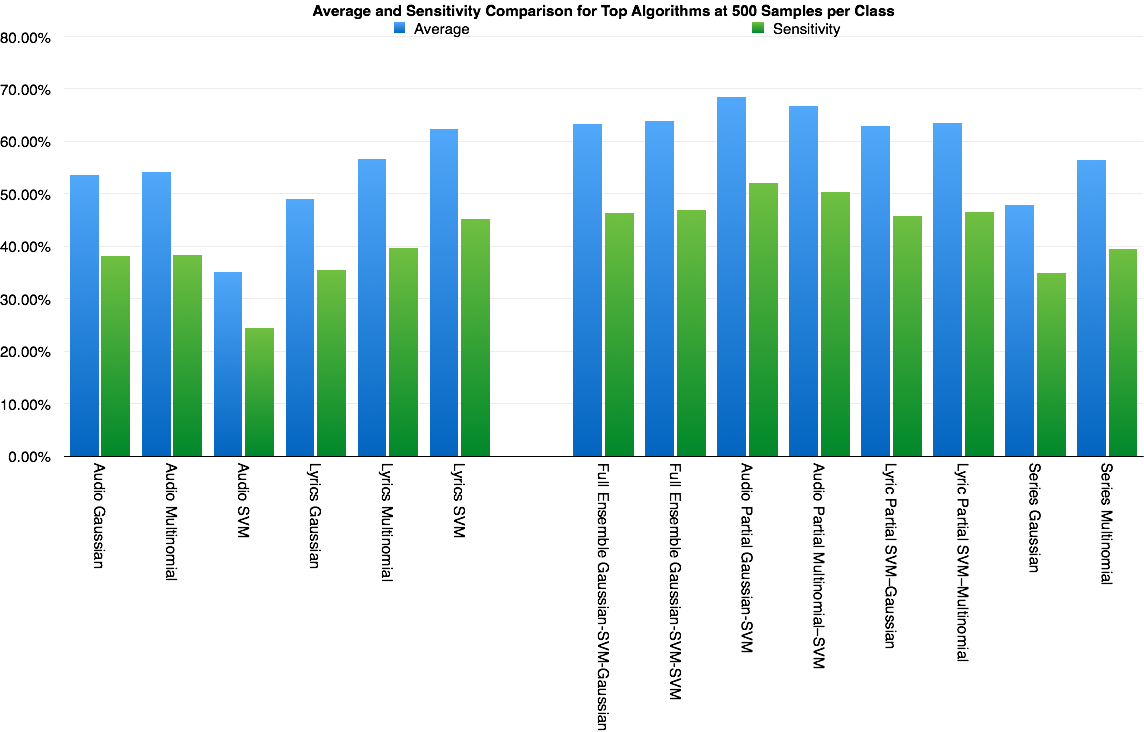
\includegraphics[width=1\textwidth]{Comparison.png}
\caption{Average and Sensitivity Comparison for Top Algorithms at 500 Samples per Class. The left side contains the accuracies and sensitivity values for the unimodal classifiers. The right side contains the accuracies and sensitivity values for the top multimodal classifiers for each configuration.}
\end{figure}

Figure 5.1 shows the performance of the top classifiers and the top benchmarks using 500 training sample per class. 
It provides a good understanding of what configurations are most effective. Figure 5.2 contains the learning curve of some 
of the top classifiers for both unimodal and multimodal. Some of the unimodal classifier perform better at smaller datasets. However once the 
dataset reaches 500 samples per class,  all the multimodal classifiers surpass the unimodal ones. Figure 5.2 also suggests that the training sizes used are not enough
to overfit the data since the slope form most of the curves is increasing for all the points displayed. This behavior indicates that 
a larger dataset should provide better accuracies for many of these algorithms. 


\begin{figure}
 \centering
 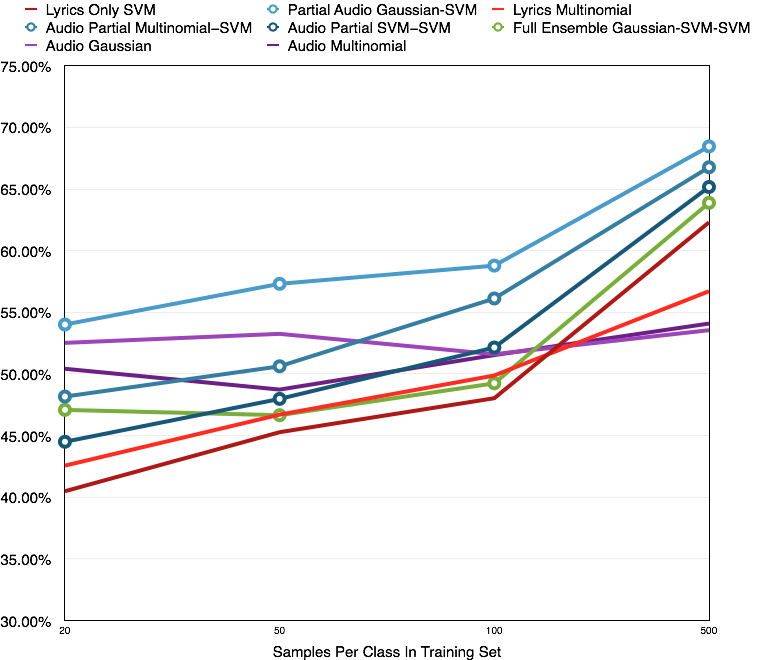
\includegraphics[width=\linewidth]{LearningCurves.png} 
 \caption{Learning Curves for Top Unimodal and Multimodal Classifiers. Plain lines represent unimodal classifiers. While the lines with circles represent the multimodal classifiers. }
\end{figure}

\section*{Better Reliability}

Both the sensitivity and the variance serve as a good indication of the reliability of the system.
A multi-class classification algorithm could possibly have strong average 
recognition accuracy as a result of performing really well for one class but 
poorly for the others.  A high average and a high variance is highly indicative of this case. However,
a high sensitivity or a high average paired with a low variance indicate that the classifier is 
both reliable and accurate. 

Table 5.2 shows the average confusion matrices for the top 
two fusion algorithms and the top three benchmarks. The columns represent 
the true label "H", "S", "A" for the classes happy, sad and angry. The rows 
represent the algorithm's prediction "h", "s", "a" for happy, sad and angry.

Table 5.2 is very informative in terms of what classes are harder to recognize. 
Clearly, happy songs pose a greater challenge than angry songs. This makes 
sense because angry words tend to only be present in angry music. For example 
words like "wrath" or "rage" are more indicative of emotion than words like "sunny" or "cheer".
 The same occurs with the Sad classification, but to a lesser extent.
 
 Consider how  the accuracy for angry songs remains relatively constant throughout all the experiments,
but the accuracy for happy songs plummets in Table 5.2.d and Table 5.2.e. Table 5.2.e shows that the audio-only Gaussian 
classifier incorrectly selects the angry classification for 56.77\% of happy songs and for 39.03\% of sad songs. 
 This behavior is evidence that the angry class is getting over-classified, since a disproportionate number of 
 songs receive that classification.  Similarly Table 5.2.d assigns happy songs
 to one of the three classes with almost equal probability, which suggests the classifier cannot identify this class as well as
 others. 
 
These  issues are at play in the case of unimodal classifiers, which would be undesirable for
real world applications. As seen in Table 5.2.a and Figure 5.2.b,  
multimodal classifiers can identify happy songs more accurately without any noticeable loss in angry classification. 
Additionally these classifiers do not select a particular class in a disproportionate manner. 




\begin{table}
\centering 
\subfigure[Audio Partial Gaussian-SVM]{
		\begin{tabular}{l |c|c|c|}
			 & H & S & A\\
			\hline
			h & \textbf{58.93\%} & 15.60 \% &16.97\% \\
			\hline
			s & 19.93\% & \textbf{73.07 \%} & 9.67\% \\ 
			\hline
			a & 21.13\% &11.33 \% & \textbf{73.37\%} \\
			\hline
		\end{tabular}
	}
\subfigure[Audio Partial Mutimodal-SVM] {
	\begin{tabular}{l |c|c|c|}
	 & H & S & A\\
	\hline
	h & \textbf{58.70\%} & 19.00 \% &17.80\% \\
	\hline
	s & 18.70\% & \textbf{67.10 \%} & 7.70\% \\ 
	\hline
	a & 22.60\% &13.90 \% & \textbf{74.50} \\
	\hline
	\end{tabular}
}
\subfigure[Lyrics SVM]{
		\begin{tabular}{l |c|c|c|}
			 & H & S & A\\
			\hline
			h & \textbf{52.83\%} & 19.77 \% &17.27\% \\
			\hline
			s & 23.13\% & \textbf{63.93 \%} & 12.60\% \\ 
			\hline
			a & 24.03\% &16.30 \% & \textbf{70.13\%} \\
			\hline
		\end{tabular}
}
\subfigure[Lyrics Multinomial]{

	\begin{tabular}{ l |c|c|c|}
	 & H & S & A\\
	\hline
	h & \textbf{36.93\%} & 13.37 \% &7.87\% \\
	\hline
	s  & 32.23\% & \textbf{59.27 \%} & 18.20\% \\ 
	\hline
	a & 30.83\% &27.37 \% & \textbf{73.93} \\
	\hline
	\end{tabular}
}

\subfigure[Audio Gaussian]{

	\begin{tabular}{ l |c|c|c|}
	 & H & S & A\\
	\hline
	h & \textbf{24.23\%} & 7.80 \% &7.53\% \\
	\hline
	s  & 19.00\% & \textbf{53.17 \%} & 9.20\% \\ 
	\hline
	a & 56.77\% &39.03 \% & \textbf{83.27} \\
	\hline
	\end{tabular}
}

\caption{Confusion Matrices for Top Fusion and Top Benchmarks.  Sub-tables (a) and (b) show that top fusion classifiers are more accurate and reliable than the top unimodal classifier in sub-table (b). Sub-tables (d) and (e) show the most prominent issues found in unimodal classifiers. The column 'H' in sub-tables (d)  shows that the classifier is making random choices to classify the happy class. The row 'a' in table (e) shows that the classifier is over-classifying songs as angry. }
\end{table}


\chapter{Conclusion}

Through the experiments and results presented in this research, we have reached the conclusion that 
multimodal classifiers improve both the accuracy and the robustness of the process.  We 
determined that some sentiments are harder to identify. It was also demonstrated that the recognition of these
challenging sentiments can be improved greatly through multimodal classification without having a significant 
impact on the accuracy of other classes. 


Although many configurations were introduced, the most promising were the Partial Lyric and the Partial
Audio architectures. These two groups dominated the ranks of the top ten in both accuracy and Sensitivity. 
All comparison metrics reached the conclusion that the Partial Audio architecture with an initial Gaussian classifier followed
by an SVM with histogram intersection as a kernel is the strongest classifier.  



\chapter{FUTURE WORK}
We explored the benefits of combining classification methods in 
different configurations.  The features used for 
the paper underlined the added benefit of multimodal 
classification. Possible future work includes using more complex features that 
take into account sentence semantics to capture word modifiers. Another 
possible route for improvement on this paper would be to extend the number 
of classes used to all six Ekman emotions. 


